\documentclass[twocolumn,5p]{elsevier}
\usepackage{custom}

\begin{document}
\title{Accelerating Research with AWS IoT}
\author{Bruno~?, Marcillo~?, Brent~Maranzano, Giuseppe~Cogoni}

\begin{abstract}
Abstract
\end{abstract}

\maketitle
\tableofcontents

\section{Background}
\label{sec:background}

The speed of designing synthetic routes and defining formulations for new drug
substances can be limited by the rate at which the data becomes available for
decision making. Much of the data is generated by offline laboratory
experiments, which requires process sampling, subdividing, transporting and
consequently time-consuming sample preparation prior to analysis, in addition
to the time to analyze, interpret and report the results. An obvious path to
accelerate sample measurements is to increase the number of analyses that can
be performed in parallel by either increasing the staff or through automation.
Alternatively, the entire process can be shortened by performing the analysis
in-situ. This approach, referred to as Process Analytical Technology (PAT), has
been used in the pharmaceutical industry for decades, but has been limited to
monitoring a few key parameters, most commonly using spectroscopic tools. The
advent of miniature, cheap electronics coupled with the Internet of Things
(IoT) has opened the possibility of monitoring a wide range of parameters in
real-time. The one obstacle that has inhibited the widespread adoption of IoT
in the pharmaceutical industry is the lack of a secure, scalable and
cost-effective platform that can be used to store, analyze and visualize the
data. In this paper, we describe the development of a combination of on-premise
and cloud-based IoT platform that can be used to monitor and analyze data from
a wide range of sensors. The platform is designed to be scalable, secure and
cost-effective, and is demonstrated by monitoring the crystallization of a drug
substance in real-time.

\section{Architecture}
\label{sec:architecture}

The key to a successful IoT platform is the ability to scale to a large number
of devices that can be readily implemented in various processes with minimal experience or training by the end user e.g. ``plug-n-play". This minimal training interface often requires
developing custom in-house applications that make calibration, measurement and analysis
simple and robust. Moreover, the IoT platform must handle the large amount of
data generated by the sensors securely and cost-effectively. The architecture


\begin{figure}[ht] 
    \centering
    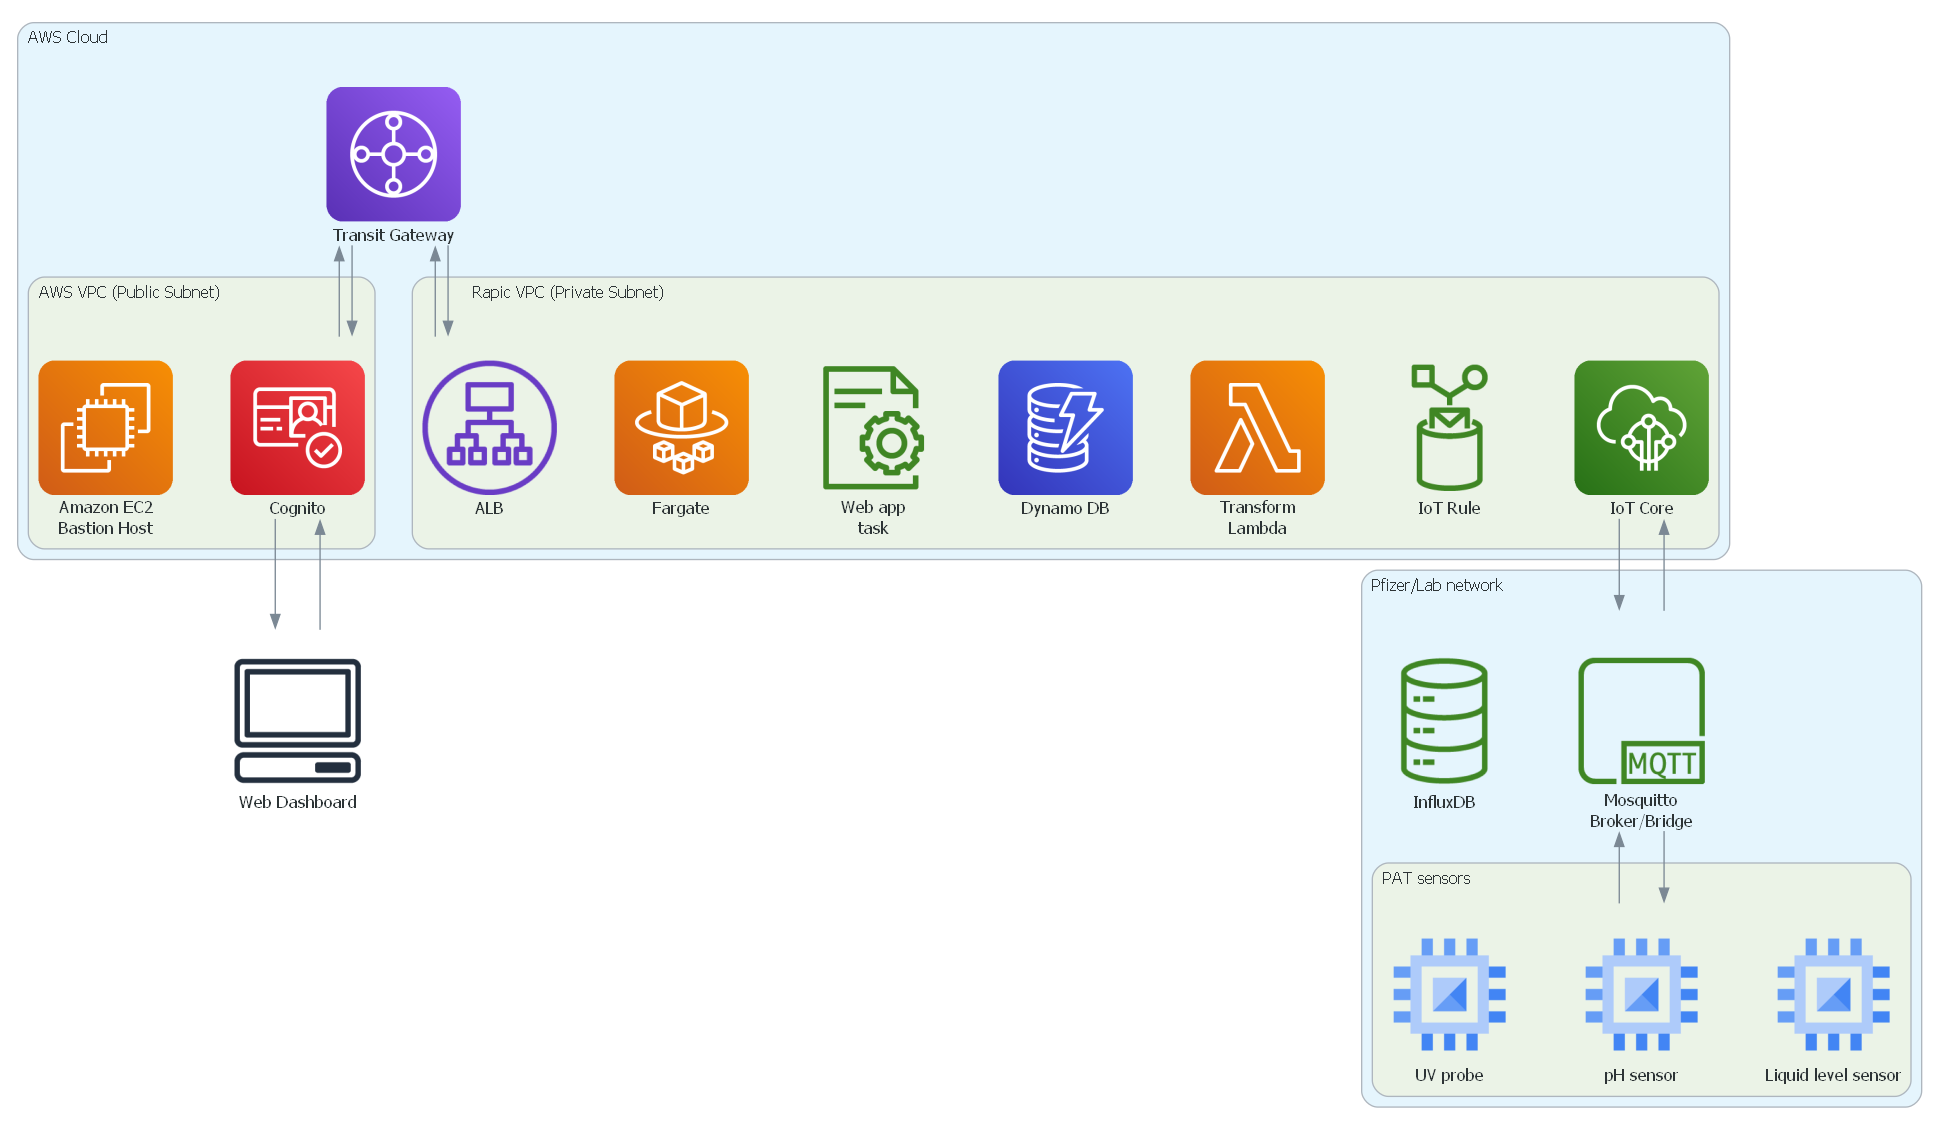
\includegraphics[width=0.7\columnwidth]{./img/architecture.png}
    \caption{Figure caption.
    \label{fig:architecture}}
\end{figure}

\begin{comment}
\section{Data}
\label{sec:data}
Referent to \ref{fig:mypicture}.

% multicolumn

\begin{equation}
     \frac{d}{dt}\left( mv \right)_{\textrm{sph}}
        = F_{\textrm{el}} \left ( \delta \right ) 
        + F_{\textrm{dis}} \left ( \dot{\delta} \right )
        - F_{\mathrm{grav}}
    \label{eq:sphere_motion}
\end{equation}

\begin{tabular}{ |l|l| }
  \hline
  \multicolumn{2}{|c|}{Team sheet} \\
  \hline
  GK & Paul Robinson \\
  LB & Lucus Radebe \\
  DC & Michael Duberry \\
  DC & Dominic Matteo \\
  RB & Dider Domi \\
  MC & David Batty \\
  MC & Eirik Bakke \\
  MC & Jody Morris \\
  FW & Jamie McMaster \\
  ST & Alan Smith \\
  ST & Mark Viduka \\
  \hline
\end{tabular}

%multirow table
\begin{table}[ht]
    \begin{center}
    \begin{tabular}{l l r}
    \hline \hline
    multirowname & column2 & column3 \\
    \hline
    \multirow{4}{*}{name1} 
        & r1c1 & r1c2 \\
        & r2c1 & r2c2 \\ \hline
    \hline \hline
    \end{tabular}
    \end{center}
    \caption{Table caption. \label{tab:polymer_spheres}}
\end{table}

\begin{figure}[ht] 
    \centering
    \includegraphics[width=0.7\columnwidth]{./img/mypicture.png}
    \caption{Figure caption.
    \label{fig:mypicture}}  
\end{figure}

%cell alignment using specific character
\begin{table}[ht]
    \begin{center}
    \begin{tabular}{l r@{$\pm$}l}
    \hline \hline
    parameter & mean & std \\
    \hline
    parameter1 (units) & mean&std \\
    parameter2 (units) & mean&std \\
    \hline \hline
    \end{tabular}
    \end{center}
    \caption{Table caption \label{tab:crystal_parameters}}
\end{table}

\begin{itemize}
  \item The first bullet
  \item The second bullet
  \item The third etc \ldots
\end{itemize}

\begin{enumerate}
  \item The first item
  \item The second item
  \item The third etc \ldots
\end{enumerate}

\begin{description}
  \item[First] The first item
  \item[Second] The second item
  \item[Third] The third etc \ldots
\end{description}

\section{appendixAdditional}
\label{sec:appendixAdditional}

\includepdf[pages={-}]{otherFile.pdf}

\begin{lstlisting}[language=Python]
    #Python Code
\end{lstlisting}

\onecolumn

\begin{center}
\includemedia[
  label=medialabel,
  addresource=./img/videofile.mp4,
  activate=pageopen,
  width=5cm, height=7cm,
  flashvars={
     source=./img/videofile.mp4
    &loop=true
  }
]{\includegraphics[width=1.0\textwidth]
{./img/videopicture.png}}{VPlayer.swf} \\
\end{center}

\begin{comment}
Comments
\end{comment}

\listoffigures
\bibliographystyle{model1a-num-names}
\bibliography{referencesmaster}

\end{document}
